\chapter{Syntaktická a sémantická analýza kódu}
Abychom mohli implementovat náš jazyk (MonkeyC), je potřeba vytvořit aplikaci, která je schopna číst "věty" na vstupu a odpovídajicím způsobem rozpoznává klíčová slova či fráze naší gramatiky.(Obecně je jazyk složení platných vět, kdy věta se skládá z frází a fráze se skládá ze symbolů slovní zásoby).\\
Obecně lze říci, pokud nějaká aplikace vykonává (interpretuje) zápis jiného programu v jeho zdrojovém kódu ve zvoleném programovacím jazyce (v našem případě Typescript), že se jedná o tzv. interpret \cite{Interpret_2020}. Jako příklady uvedu kalkulačku, aplikace pro čtení konfiguračních souborů, Python interprety, atd... Pokud, na druhou stranu, převádíme "věty" z jednoho jazyka do druhého (např. z Javy do 'C Sharp'), nazýváme takovou aplikaci překladačem.\\
Úkolem překladače či interpreta je tedy rozpoznat platné vstupy, tedy věty, fráze, subfráze, klíčová slova, atd... Přičemž rozpoznáním platného vstupu je myšleno identifikovat jednotlivé fráze a rozližit je od jiných.\\
Jako příklad použijeme rozpoznání vstupu $input = 1;$ s validní MonkeyC syntaxí.  Víme tedy, že "input" je cíl přiřazení a "1" představuje hodnotum která se má přiřadit. Stejně jako jsme my schopni rozližit v našem jazyce sloveso od podstatného jména, je naše aplikace schopna rozlišit toto přiřazení od např. importu knihovny pomocí klíčového slova "using".\\
Programy, které jsou schopny rozpoznávat konkrétní jazyk, se nazývají parsery nebo syntaktické analyzátory, přičemž syntax odkazuje na pravidla obsažená v popisu jazyka, čili gramatice.\\

\begin{figure}
	\centering
	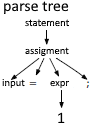
\includegraphics[scale=1.5]{images/assigment}
	 \caption{přiřazení hodnoty 1 proměnné input}
	 \label{img:assigment}
\end{figure}


\section{ANTLR - Nástroj pro generování překladače}
ANTLR nebo také ANother Tool for Language Recognition (jiný nástroj pro rozpoznávání jazyka) \cite{ANTLR_2021} je výkonný nástroj pro generování syntaktických analyzátorů, tzv. "parser". Tento parser je poté schopen číst, zpracovávat, spouštět nebo překládat strukturované textové či binární soubory. Použivá se především k vytváření nových jazyků, nástrojů nebo "frameworků". Využívá bezkontextový jazyk typu LL.
\subsection{LL syntaktický analyzátor}
LL \cite{LL_2017} je syntaktický analyzátor shora-dolů pro bezkontextové gramatiky. Analyzuje vstup zleva (Left) doprava a konstruuje nejlevější derivaci (Leftmost) věty. Gramatiky, které jsou takto analyzovatelné, se nazývají LL gramatiky.

\section{Syntaktický strom}
Syntaktický strom představuje datovou strukturu, kterou ANTLR vytvoří při parsování vstupního souboru. Struktura je složená z kořene (root) a uzlů, které mohou představovat buď další podstromy, které odpovídají pravidlům gramatiky, nebo listy stromu.\\ 
V naší aplikaci Syntaktický strom představuje třída AST (viz. kód níže), která uchovává všechna důležitá data pro korektní analýzu vstupního souboru, např. počet uzlů stromu, soubor vztahující se ke konkrétnímu stromu, kořen stromu, atd...

\begin{figure}
	\centering
	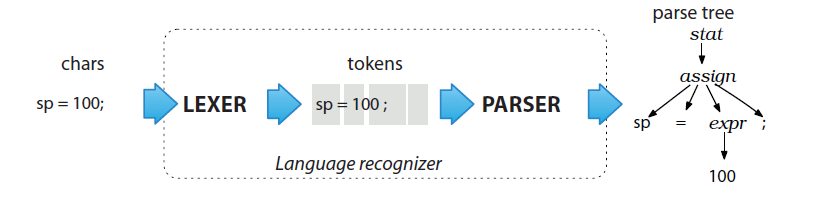
\includegraphics[scale=0.7]{images/parser}
	\caption{Ukázka, jak Language recognizer zpracovává vstupní sekvenci znaků} 			    \cite{ANTLR_PG_10}
	\label{img:parser}
\end{figure}

\lstinputlisting[label=code:AST_TS,caption={třída AST v jazyce Typescript}]{SourceCodes/AST.ts}

Další, neméně důležitou, třídou v naší apikaci je třída Node, která představuje uzel stromu. Jedná se, ve své podstatě, o strukturu uchovávající následující atributy:\\
\begin{enumerate}
	\item kontext daného uzlu
	\item předka uzlu
	\item potomka uzlu
	\item hodnotu přestavující text v daném uzlu
	\item typ uzlu, který se odvíjí od pravidel v gramatice
\end{enumerate}

\lstinputlisting[label=code:Node_TS,caption={třída Node v jazyce Typescript}]{SourceCodes/Node.ts}


\section{ANTLR Listener a callback funkce}
ANTLR disponuje dvěma mechanismy, které umožňují průchod stromem (tzv. "tree-walking mechanisms"). Jedná se o mechanismy \textbf{listener} a \textbf{visitor},pričemž výchozím je listener. Největší rozdíl mezi nimi spočívá v tom, že listener metody jsou volány nezávisle ANTLR objektem, zatímco visitor metody vyvolávají rovněž metody potomků uzlu, na kterém se právě nachází, což způsobuje, že některé podstomy nebudou při průchodu vůbec navštíveny. Samotné listenery jsou ekvivalentí SAX objektům, které se používají v XML parserech.\\
Aby bylo možné stromem procházet a při průchodu vyvolat odpovídající události, ANTLR dispinuje třídou ParseTreeWalker. Právě ona se stará o to, aby byly volány callback funkce. Další důležitou komponentou, vygenerovanou ANTLR nástrojem je rozhraní ParseTreeListener (v našem případě MonkeyCListener \ref{img:generated_files}). Toto rozhraní definuje veškeré metody potřebné k kompletnímu průchodu stromem, např. "enterEveryRule(context: ParserRuleContext)" či "exitStatement(context: StatementContext)". Ve chvíli kdy ParseTreeWalker narazí na příslušný uzel, vyvolá odpovídající metodu. TODO: příklad kdy narazí na nějaké assign třeba


\section{Sémantický strom}
Strom, jenž hraje zásadní roli v procesech, jako je našeptávání kódu, detekci chyb, kdy je použita třída z modulu, který není referencován, atd...

\section{parser}
Fusce nibh. Sed ut perspiciatis unde omnis iste natus error sit voluptatem accusantium doloremque laudantium, totam rem aperiam, eaque ipsa quae ab illo inventore veritatis et quasi architecto 
beatae vitae dicta sunt explicabo. Quis autem vel eum iure reprehenderit qui in ea voluptate velit esse quam nihil molestiae consequatur, vel illum qui dolorem eum fugiat quo voluptas nulla pariatur? Etiam ligula pede, sagittis quis, interdum ultricies, scelerisque eu. Maecenas sollicitudin. Cras pede libero, dapibus nec, pretium sit amet, tempor quis. Integer vulputate sem a nibh rutrum consequat. Pellentesque sapien. Pellentesque arcu. Suspendisse nisl. Fusce consectetuer risus a nunc. Etiam dui sem, fermentum vitae, sagittis id, malesuada in, quam. Cum sociis natoque penatibus et magnis dis parturient montes, nascetur ridiculus mus. Nam quis nulla. Nulla non lectus sed nisl molestie malesuada. Duis viverra diam non justo. Sed ac dolor sit amet purus malesuada congue. Aenean id metus id velit ullamcorper pulvinar. Aliquam ornare wisi eu metus. Neque porro quisquam est, qui dolorem ipsum quia dolor sit amet, consectetur, adipisci velit, sed quia non numquam eius modi tempora incidunt ut labore et dolore magnam aliquam quaerat voluptatem.

\endinput
